% !TEX root = ../main.tex

\chapter{绪论}

\section{研究背景与意义}

金融异常检测面对的是具体业务对象。它可能是一笔金额和地域组合异常的交易，也可能是账户在短时间窗内突然改变的行为序列，或由设备指纹、登录地点和交易对手共同构成的高风险模式。在实际检测系统中，检测效果与执行效率共同构成业务约束\citep{aggarwal2017outlier,song2024financialriskstgnn}。吞吐不足会造成请求堆积，尾延迟过高则可能使告警错过处置窗口，高频交易流持续进入系统后，风险告警必须在有限时间内完成。

图~\ref{fig:fin-ad-business-scene}概括了本文所关注的业务环境。单笔交易特征、账户时间窗统计、设备与地域信息以及关系结构特征需要在进入检测链路前形成一致的输入表达；异常分数和风险排序又要及时返回上层业务。这里不展开金融行业的一般流程，关键约束只有两个：输入持续增长，告警时间预算有限。前者抬高计算与存储压力，后者限制了系统依靠离线批处理消化峰值流量的空间\citep{pei2021gpudatabase,zhang2023gpuolap}。

\begin{figure}[!b]
  \centering
  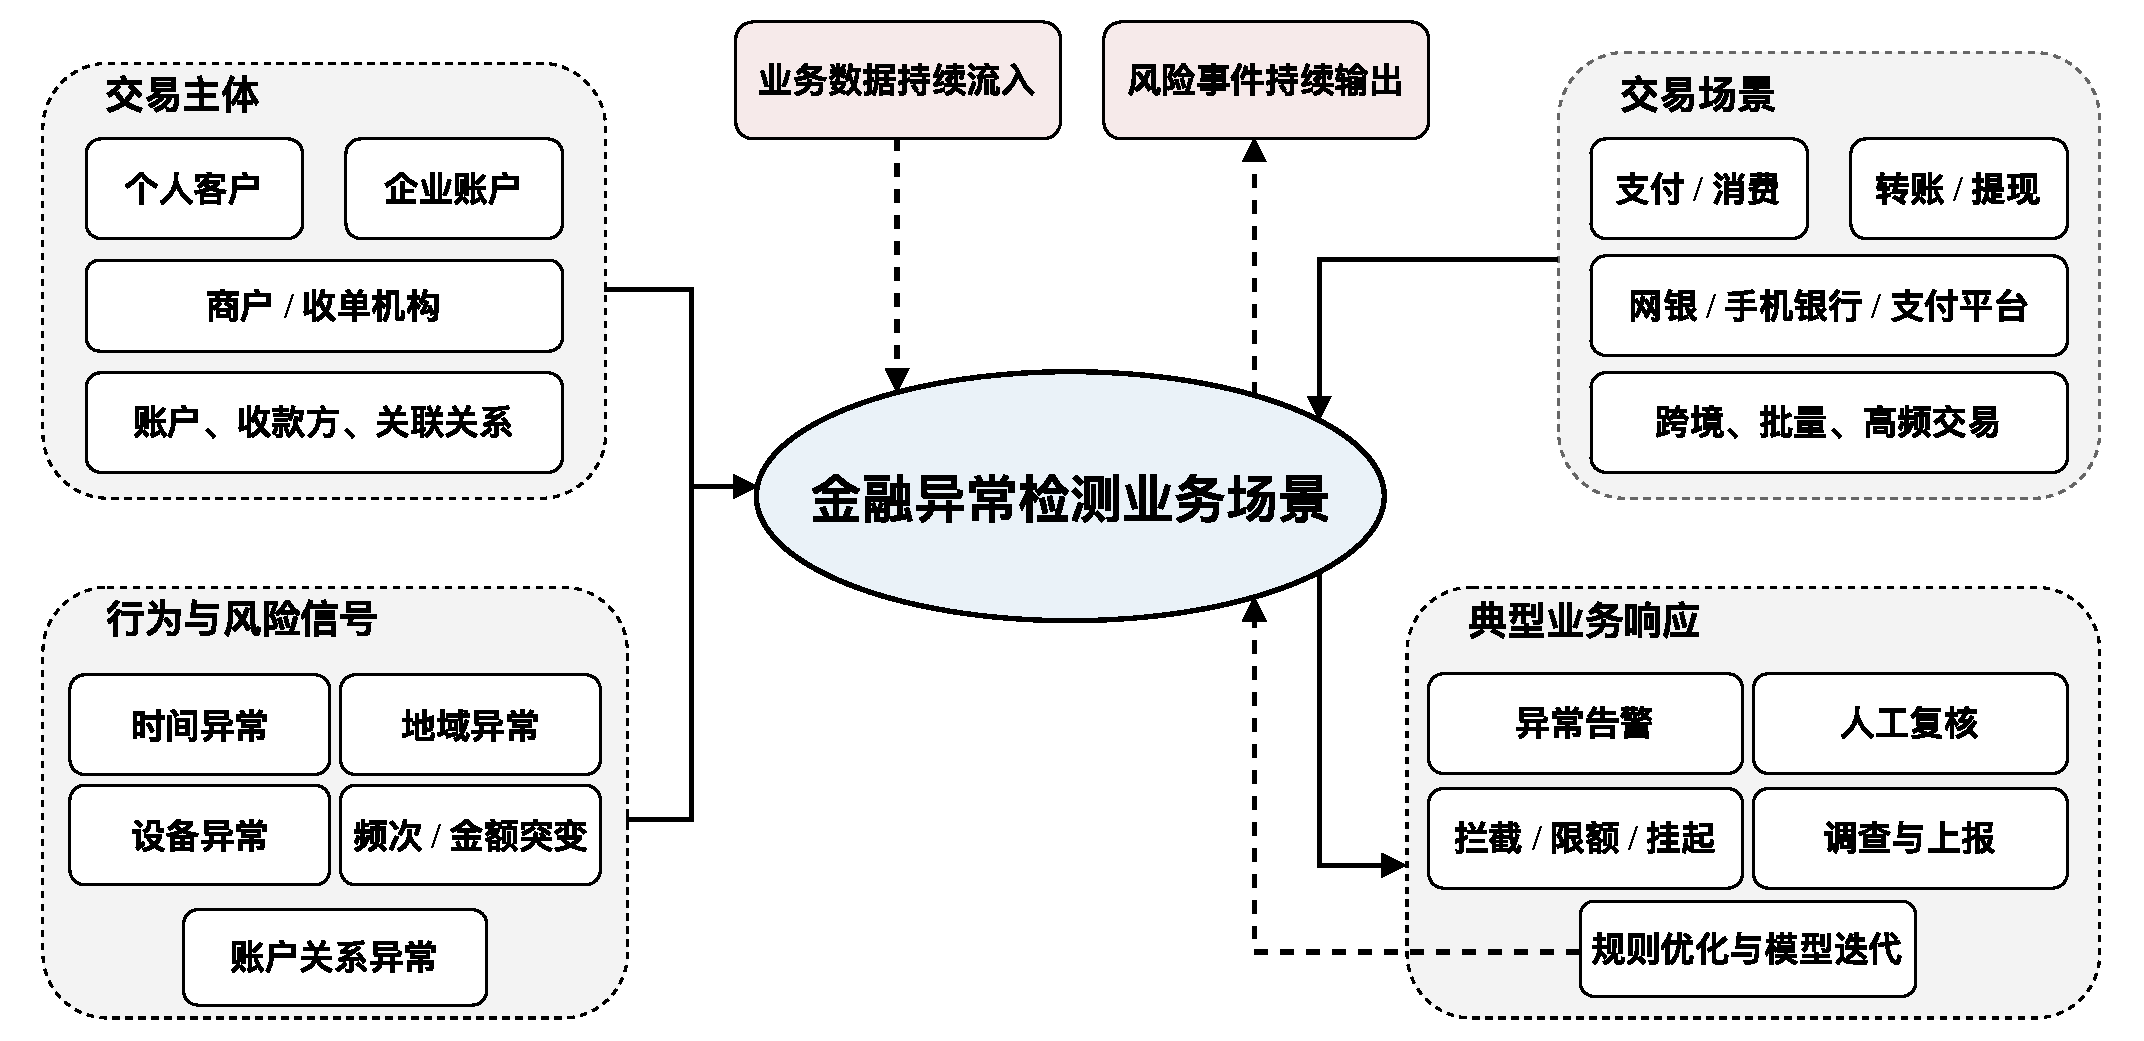
\includegraphics[width=0.95\linewidth]{figures/fig1-1_financial_anomaly_business_scene.pdf}
  \caption{金融异常检测业务场景总览图（本文绘制）}
  \label{fig:fin-ad-business-scene}
\end{figure}

数据规模较小时，主要矛盾通常是 CPU 上的距离计算、排序和聚合耗时。将评分算子迁移到 GPU 后，主导瓶颈随之转移。全量距离或近邻计算仍可能产生远大于输入矩阵的中间结果；查询向量和候选结果跨越 CPU--GPU 边界时会产生 H2D、D2H 传输；候选 ID、距离与排序信息若在主机侧重新组织，还会增加同步点。索引无法完全驻留显存时，SSD 访问开始进入关键路径。扩展到多 GPU 后，结果归并以及 PCIe、NUMA 和共享 I/O 竞争又会限制新增计算资源的利用率。

图~\ref{fig:scale-bottleneck-migration}描述了主导因素随系统规模和执行环境发生的变化。小规模阶段缩短 CPU 算子时间即可得到明显收益；当评分已经 GPU 化，系统开始受数据驻留位置和模块边界影响；当单卡链路被压缩，多 GPU 调度、跨卡归并与共享 SSD 路径才成为新的上限。只优化某个检测器或检索算子，无法保证端到端吞吐同步提高\citep{song2026vectoranns,li2024multigpunuma}。

\begin{figure}[!tb]
  \centering
  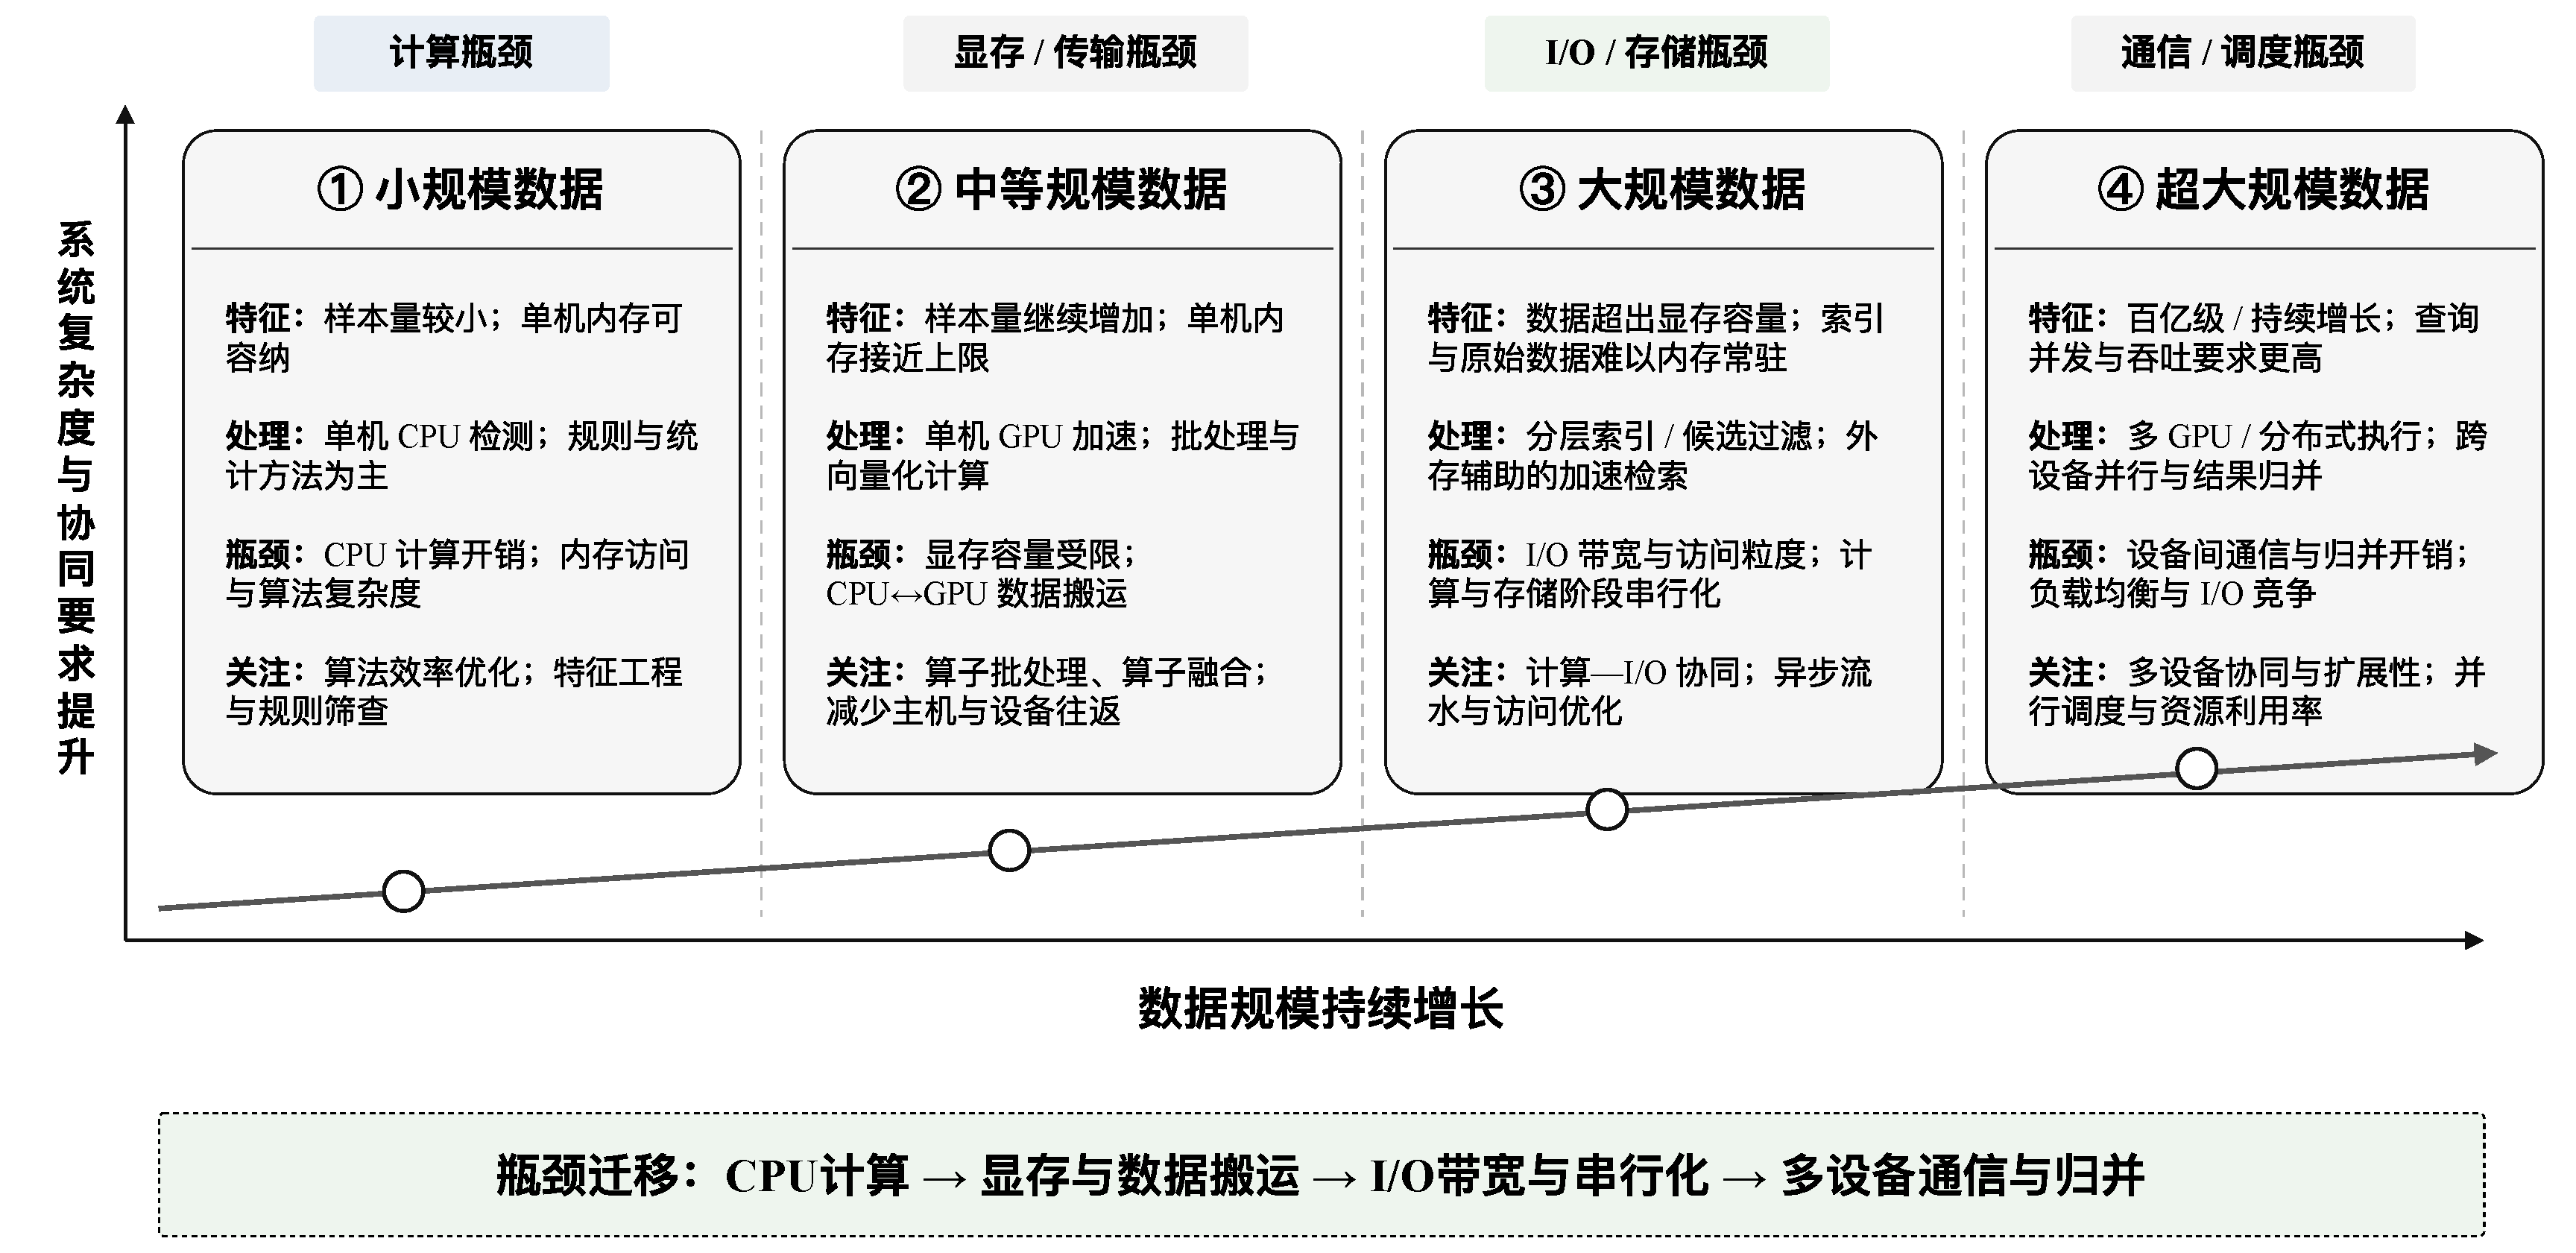
\includegraphics[width=0.90\linewidth]{figures/fig1-2.pdf}
  \caption{数据规模增长与系统瓶颈迁移示意图（本文绘制）}
  \label{fig:scale-bottleneck-migration}
\end{figure}

全量评分成本过高，使两阶段处理成为一种可行的系统选择：先通过近似最近邻（Approximate Nearest Neighbor，ANN）检索得到规模受控的候选集合，再在候选集合上执行较精细的异常评分。候选召回压缩了评分范围，但也引入了新的取舍。候选预算过小可能遗漏与异常判断有关的邻域，预算过大又会把计算压力重新交给评分模块。更重要的是，近似最近邻搜索与张量化评分的简单串接并不会自动形成低开销链路。候选结果若返回 CPU 打包，再通过 H2D 送入 GPU 评分，局部算子的加速仍可能被阶段边界抵消。

本文据此构建 FlashTOD。系统以 PyTOD 作为候选集合上的张量化异常评分模块\citep{zhao2022tod}，以已有 FlashANNS 系统的外存 ANNS 能力作为大规模候选召回前端\citep{xiao2025flashanns}。单 GPU 部分研究查询、候选和评分中间张量如何连续留在设备侧；多 GPU 部分研究查询调度、结果归并和共享 I/O 约束。本文讨论的是这些已有能力在金融大规模异常检测链路中的协同组织与实现边界，不将其表述为新的异常检测理论模型，也不把当前实验结果外推为对全部金融风控部署条件的普遍结论。

\section{本文研究内容}

\subsection{本文研究对象与系统处理链路}

图~\ref{fig:fin-ad-standard-flow}展示了金融异常检测所处的完整业务流程，其中包含数据接入、特征处理、风险识别、告警以及后续处置。该图用于交代系统上下文，并不表示本文实现了银行生产风控的全部环节。真实生产链路还可能包含规则引擎、人工审核、工单流转、拦截或冻结、额度调整以及模型在线更新闭环，这些环节依赖机构规则、权限体系和持续运营机制，不属于本文实现范围。

本文从数据预处理完成后的向量化输入开始，重点覆盖候选召回、候选组织、PyTOD 异常评分、风险排序和必要结果输出。原始交易记录、账户时间窗行为、设备与地域特征或图关系统计在进入系统前被整理为固定维度向量；候选召回前端返回候选 ID、距离和索引映射信息；评分模块在候选集合上生成异常分数与排序；系统只把最终小规模结果和必要日志交给后续业务。这里的“结果输出”不包含规则决策、人工审核和业务处置本身。

\begin{figure}[!htbp]
  \centering
  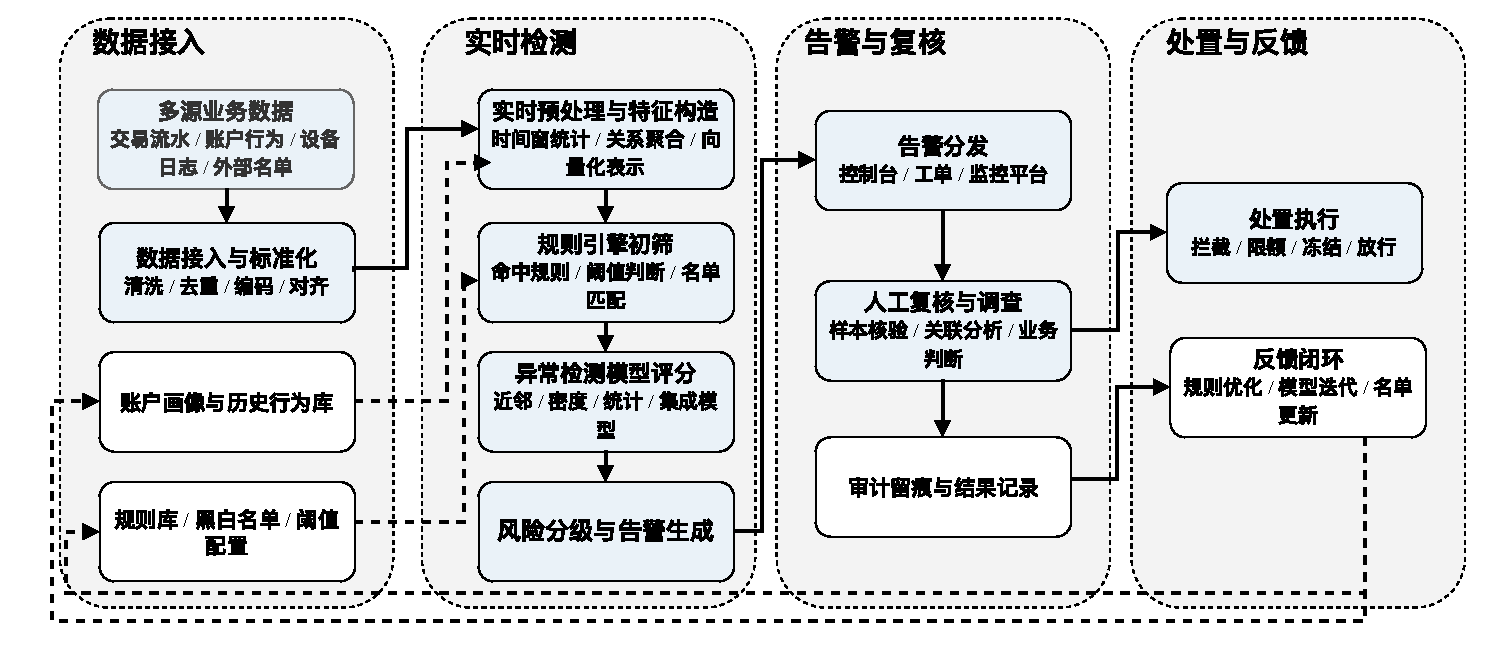
\includegraphics[width=\linewidth]{figures/fig1-3_financial_anomaly_standard_flow.pdf}
  \caption{金融大规模异常检测系统标准处理流程图（本文根据金融异常检测流程整理绘制）}
  \label{fig:fin-ad-standard-flow}
\end{figure}

\FloatBarrier

\subsection{本文关注的核心系统问题}

上述研究范围内有四个直接影响端到端表现的问题。它们分别落在评分、召回、模块边界和多设备扩展阶段，后文的系统设计与实验验证均围绕这四类问题展开。

\paragraph{异常评分阶段的高复杂度计算问题}

距离型和密度型异常检测依赖近邻计算，常见评分过程包含距离计算、排序、局部密度估计与邻域聚合\citep{aggarwal2017outlier,zhao2022tod}。复杂度压力还来自计算过程产生的中间结果。输入矩阵本身可能仍能装入显存，但若直接构造全量距离矩阵，存储量会达到 $O(n^2)$；朴素实现中的成对差分张量还会随特征维度继续放大。问题1聚焦于避免在全量样本上物化高代价中间结果，并把可张量化评分限制在候选预算内。

\paragraph{候选召回阶段的存储访问与吞吐瓶颈问题}

索引能够驻留显存时，召回开销主要来自近邻搜索与候选维护；索引超过显存容量后，SSD 读页进入关键路径。此时搜索性能由 ANN 算法、I/O 访问粒度、在途请求数量以及 Fetch、Compute 和候选 Update 的重叠程度共同决定。候选预算同样受到两端约束：预算过小可能降低异常覆盖和 Recall@$k$，过大则增加 PyTOD 的距离、\texttt{topk} 与聚合成本。问题2研究候选质量和外存访问代价的共同控制\citep{song2026vectoranns,xiao2025flashanns}。

\paragraph{CPU--GPU 数据传输与阶段同步问题}

候选召回返回 candidate ID、distance、local rank 以及 reference/index mapping。若这些字段回到 CPU 后由主机侧 \texttt{pack\_candidates} 重新组织，执行路径会变为“GPU 检索 $\rightarrow$ D2H $\rightarrow$ CPU 候选重组 $\rightarrow$ H2D $\rightarrow$ GPU 评分”。问题出现在阶段边界。一次检索即使足够快，两轮数据搬运、对象转换和同步仍会抬高端到端时延。问题3因此聚焦设备侧候选表达和连续执行，具体定位 CPU--GPU 通信开销出现的位置\citep{pei2021gpudatabase,zhang2023gpuolap}。

\paragraph{多 GPU 扩展中的结果聚合与共享 I/O 瓶颈问题}

索引复制（replicated）使每张 GPU 保留完整索引并独立处理查询，设备间依赖较少，适合吞吐优先且索引可以复制的条件；索引分片（sharded）有利于容量扩展，却需要合并各卡局部结果。无论采用哪种组织方式，多张 GPU 都可能竞争同一 PCIe 交换路径、NUMA 远端内存或 SSD 通道。设备数量增加后，通信、归并和 I/O 排队可能同时增长，所以吞吐不会自然线性扩展。问题4研究不同部署路径的适用条件及其代价，不预先声称所有多 GPU 瓶颈已经被解决\citep{li2024multigpunuma,cuvs_multi_gpu_nn}。

表~\ref{tab:problem-method-chapter-metric}给出四个问题与后续章节的对应关系。表中指标均来自现有实验设计，没有新增实验或数值。

\begin{table}[!htbp]
  \caption{核心问题、处理方式、对应章节与验证指标}
  \label{tab:problem-method-chapter-metric}
  \centering
  \footnotesize
  \setlength{\tabcolsep}{3pt}
  \renewcommand{\arraystretch}{1.20}
  \begin{tabularx}{\linewidth}{@{}P{2.55cm}P{4.65cm}P{2.15cm}Y@{}}
    \toprule
    核心问题 & 本文主要处理方式 & 对应章节 & 主要验证指标 \\
    \midrule
    异常评分复杂度 & 候选召回压缩评分范围，PyTOD 在候选集合上执行张量化评分 & 第三章、第六章 & PR-AUC、Recall@$k$、QPS \\
    外存候选召回开销 & 接入 FlashANNS 异步 I/O---计算流水线，联动控制候选预算 & 第三章、第四章 & 检索阶段耗时、QPS、I/O 通道配置影响 \\
    CPU--GPU 往返 & GPU 主导数据路径，设备侧组织 ID、distance、rank 与索引映射 & 第四章、第六章 & 查询准备与候选组织耗时、QPS、p99 延迟 \\
    多 GPU 扩展损耗 & replicated 主方案、设备侧归并兜底路径与拓扑感知 I/O 控制 & 第五章、第六章 & QPS、p99 延迟、资源利用率、扩展倍数 \\
    \bottomrule
  \end{tabularx}
\end{table}

\subsection{本文研究边界与主线}

FlashTOD 定位于系统协同与执行路径研究，沿用 PyTOD 的评分能力，重点研究它与候选召回前端之间的系统接口、数据驻留和执行顺序。FlashANNS 属于已有 ANNS 系统；本文使用其候选检索能力，异步 I/O 机制和索引算法沿用原系统设计。RAPIDS、FAISS-GPU、页锁定内存和 NCCL 则用于 FlashTOD 的组织、适配和实现。

当前系统范围是单机单 GPU 与单机多 GPU。多机分布式索引、跨机通信和集群调度没有进入本文验证。实验使用公开真实或半真实金融数据检验两阶段链路的可用性，并使用高保真合成数据观察大规模吞吐、时延和扩展趋势；这些输入不能等同于银行生产流量。现有外部基线覆盖也不完备，结论只适用于本文的数据、硬件、候选预算和实现路径。全文的主线因而限定为三部分：FlashTOD 协同框架、单 GPU 数据路径优化和单机多 GPU 扩展。

\section{研究目标与技术路线}

本文的目标是在既定检测方法和硬件条件下，降低候选召回---异常评分链路的系统开销，并检验该链路在单机 GPU 环境中的扩展边界，共同观察检测效果、QPS 和尾延迟。

评分范围是需要压缩的对象。第三章先把金融数据整理为统一向量输入，以 FlashANNS 产生候选集合，再由 PyTOD 完成候选集上的张量化评分，对应问题1和问题2。这个阶段建立功能链路，并通过 PR-AUC、Recall@$k$ 等指标检查候选预算是否造成不可接受的效果损失。

候选集合生成后，新的瓶颈出现在模块边界。第四章把查询表示、candidate ID、distance、local rank、索引映射和评分中间张量尽量保持在设备侧，并利用异步 I/O、双缓冲和必要的页锁定内存减少等待。这里对应问题2和问题3。

当单卡链路得到压缩后，多 GPU 扩展才具有实际意义。第五章比较多GPU扩展的replicated 主方案、容量受限时的设备侧归并路径以及共享 I/O 约束，对应问题4；第六章在统一实验口径下汇总检测效果、阶段耗时、QPS、p99 延迟和资源利用率。表~\ref{tab:research_route}概括了这条路线的实现层次。

\begin{table}[htbp]
  \caption{本文技术路线的实现层次}
  \label{tab:research_route}
  \centering
  \small
  \setlength{\tabcolsep}{4pt}
  \renewcommand{\arraystretch}{1.18}
  \begin{tabularx}{\linewidth}{@{}P{3.15cm}Y P{2.2cm}@{}}
    \toprule
    技术路线环节 & 核心任务 & 对应章节 \\
    \midrule
    统一建模与向量输入 & 对齐表格型、图金融数据与两阶段接口 & 第三章 \\
    候选召回与张量化评分 & 控制候选预算，建立 FlashANNS---PyTOD 功能链路 & 第三章 \\
    单 GPU 数据路径 & 压缩 H2D/D2H、候选重组和 I/O 串行等待 & 第四章 \\
    单机多 GPU 扩展 & 组织 replicated、设备侧归并和拓扑感知 I/O 路径 & 第五章 \\
    统一实验验证 & 检验效果、吞吐、时延、资源利用率与扩展边界 & 第六章 \\
    \bottomrule
  \end{tabularx}
\end{table}

\section{本文主要工作与技术贡献}

本文完成的工作沿三条主线组织。

\begin{enumerate}
  \item FlashTOD 协同框架。在金融大规模异常检测的统一向量输入上，本文将 FlashANNS 候选检索能力和 PyTOD 张量化评分组织为两阶段执行链路，并明确查询向量、候选 ID、distance、local rank、reference/index mapping 与评分张量之间的接口。贡献落在对PyTOD和FlashANNS研究，进行系统组织、适配、实现与验证。
  \item 单 GPU 数据路径优化。本文针对“GPU 检索---CPU 重组---GPU 评分”的折返路径，设计 GPU 主导执行链路，使候选结果和评分中间张量尽量保持在GPU侧，并结合异步 stream、双缓冲、页锁定内存及 RAPIDS 数据后端降低必要边界开销，进一步优化数据路径。值得注意的是，FAISS-GPU 用于前期 device/host pointer 路径和候选接口验证，不作为最终外存召回主路径。
  \item 单机多 GPU 扩展。本文在索引可复制时采用 replicated 查询级并行，以 CPU 控制面完成请求调度；容量受限时讨论设备侧归并和 NCCL 通信，并用 topology-aware I/O 约束共享 PCIe、NUMA 与 SSD 路径。多GPU扩展是工程实践的一个典型思路，该部分贡献落在对这些机制在 FlashTOD 中的部署组织和实验验证。
\end{enumerate}

\section{论文组织结构}

全文从表~\ref{tab:problem-method-chapter-metric}中的四个核心系统问题展开。第三章先完成 FlashTOD 的任务建模、候选召回和评分链路，主要处理问题1和问题2；第四章进入单 GPU 热路径，继续处理外存召回以及 CPU--GPU 阶段边界，对应问题2和问题3；第五章讨论 replicated、设备侧归并和共享 I/O，对应问题4。第六章把四类问题放回统一实验口径下验证，第七章总结结论与研究边界。图~\ref{fig:chapter-logic}给出了问题与章节之间的逻辑关系。

\begin{figure}[!htbp]
  \centering
  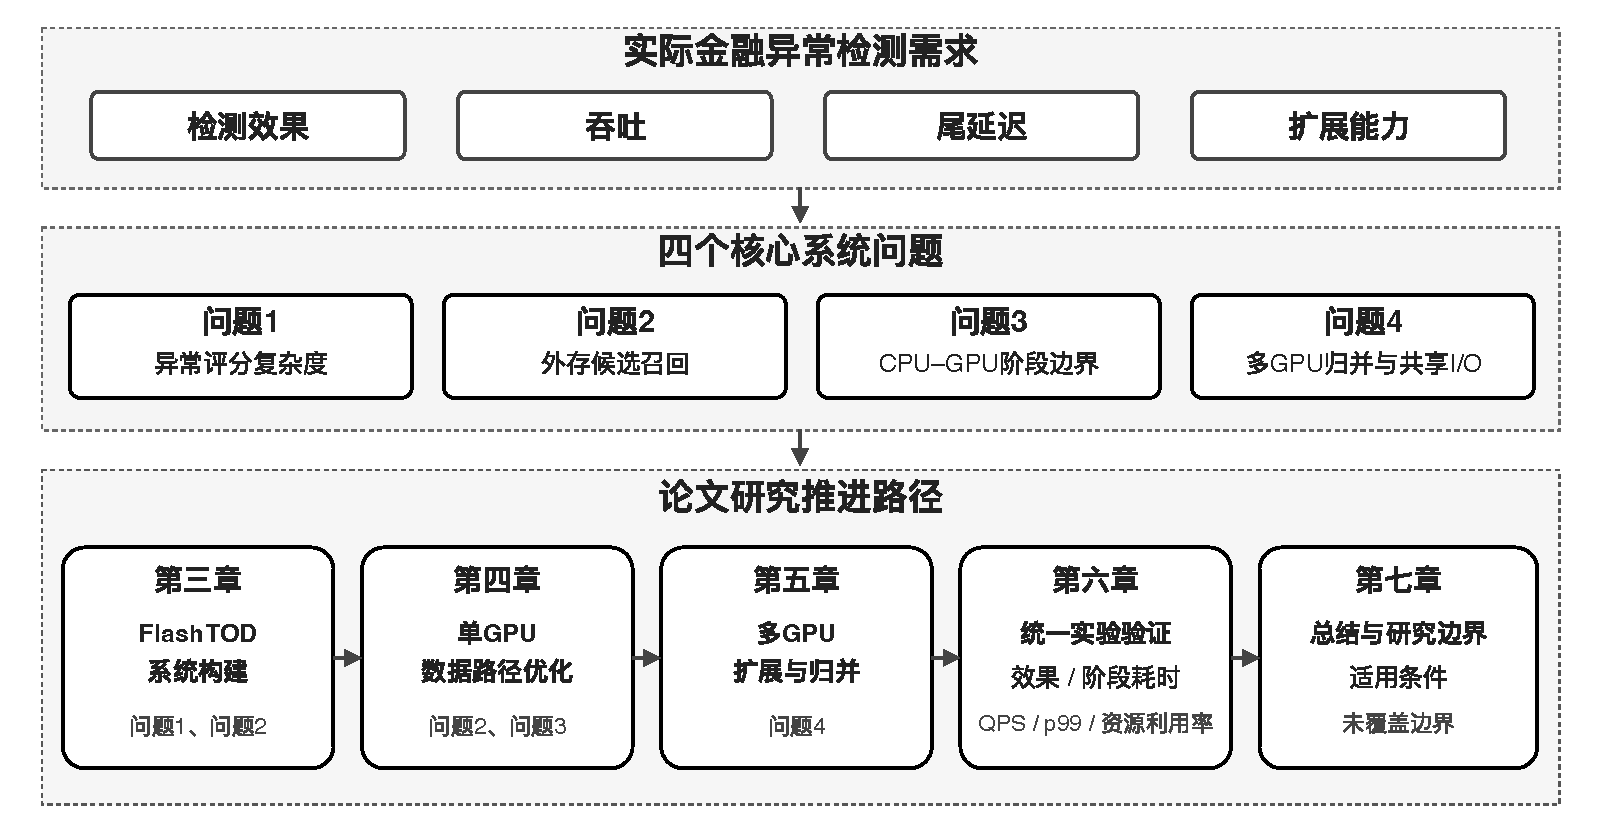
\includegraphics[width=\linewidth]{figures/fig1-4.pdf}
  \caption{全文研究内容与章节逻辑关系图（本文绘制）}
  \label{fig:chapter-logic}
\end{figure}
